\documentclass[conference]{IEEEtran}
\IEEEoverridecommandlockouts
% The preceding line is only needed to identify funding in the first footnote. If that is unneeded, please comment it out.
\usepackage{cite}
\usepackage{amsmath,amssymb,amsfonts}
\usepackage{algorithmic}
\usepackage{graphicx}
\usepackage{textcomp}
\usepackage{xcolor}
\usepackage[citecolor=red]{hyperref}
\usepackage{url}
\usepackage{booktabs}
\usepackage{multirow}
\def\BibTeX{{\rm B\kern-.05em{\sc i\kern-.025em b}\kern-.08em
    T\kern-.1667em\lower.7ex\hbox{E}\kern-.125emX}}
\begin{document}
\title{Browser Certificate Verification and HTTPS Exception Handling\\
{\footnotesize \textsuperscript{*}Note: Sub-titles are not captured in Xplore and
should not be used}
\thanks{Identify applicable funding agency here. If none, delete this.}
}

\author{\IEEEauthorblockN{1\textsuperscript{st} Given Name Surname}
\IEEEauthorblockA{\textit{dept. name of organization (of Aff.)} \\
\textit{name of organization (of Aff.)}\\
City, Country \\
email address}
\and
\IEEEauthorblockN{2\textsuperscript{nd} Given Name Surname}
\IEEEauthorblockA{\textit{dept. name of organization (of Aff.)} \\
\textit{name of organization (of Aff.)}\\
City, Country \\
email address}
\and
\IEEEauthorblockN{3\textsuperscript{rd} Given Name Surname}
\IEEEauthorblockA{\textit{dept. name of organization (of Aff.)} \\
\textit{name of organization (of Aff.)}\\
City, Country \\
email address}
\and
\IEEEauthorblockN{4\textsuperscript{th} Given Name Surname}
\IEEEauthorblockA{\textit{dept. name of organization (of Aff.)} \\
\textit{name of organization (of Aff.)}\\
City, Country \\
email address}
\and
\IEEEauthorblockN{5\textsuperscript{th} Given Name Surname}
\IEEEauthorblockA{\textit{dept. name of organization (of Aff.)} \\
\textit{name of organization (of Aff.)}\\
City, Country \\
email address}
\and
\IEEEauthorblockN{6\textsuperscript{th} Given Name Surname}
\IEEEauthorblockA{\textit{dept. name of organization (of Aff.)} \\
\textit{name of organization (of Aff.)}\\
City, Country \\
email address}
}

\maketitle

\begin{abstract}
HTTPS provides authentication, data confidentiality and integrity
    for secure web applications in the Internet. % such as online banking, Email, e-commerce transactions, etc.
%has played a significant role in communication security by providing encryption data integrity and entity authentication.
% It is used hundreds of million of times every day in web browsers.
In order to establish secure connections with the target website but not a man-in-the-middle attack,
a browser shows security warnings to users,
    when different HTTPS errors happen (for example,
        it fails to build a valid certificate chain,
         or the certificate subject does not match the domain visited).
Each browser implements its own design of warnings on HTTPS errors, to balance security and usability.
%Browsers report HTTPS security warnings if the certificate chain fails to validate.
%However, There is no clear industry consensus for browsers�� security strategies, and four major browsers exhibiting different warning design.
In this paper,
    we present a list of HTTPS errors,
    and investigate the browser behaviors on each error.
%To get a good understanding of the browser warnings,
% we design a wide variety of HTTPS certificate errors and investigate the browser warning behaviors in the field.
%We empirically assess whether browser security warnings are as effective as suggested by popular opinion.
Our study discloses several browser defects
     on handling HTTPS errors in terms of cryptographic algorithm, certificate revocation, certificate extension, name validation, 
        and HPKP.
%Our results suggest that browsers may treat the same certificate error differently.
%Based on our findings, we make recommendations for warning designers
   % and researches to ensure the security of HTTPS certificate ecosystem.
\end{abstract}


\begin{IEEEkeywords}
HTTPS, browser warning
\end{IEEEkeywords}

\section{Introduction}
HTTPS implements HTTP over TLS,
    and provides authentication, data confidentiality and integrity for secure web applications \cite{https-rfc}.
%It is used for hundreds of million of times every day in browsers .
    In the TLS negotiation, a browser verifies the server certificate by building a certificate chain,
    and validates the certificate subject with the domain visited.
The security of HTTPS is further enhanced by HPKP that pins the public keys of the website in browsers \cite{Evans2015rfc7469},
     and HSTS that forces browsers to visit the website only using HTTPS but not HTTP \cite{hodges2012rfc6797}.

There are various errors in the TLS negotiations and also the HTTPS security-enhancements.
Browsers show security warnings to users with different levels, on different errors:
(\emph{a}) a low-risk warning is shown in the address bar, not interrupting the browsing;
(\emph{b}) a medium-risk warning is shown as a full-screen page to interrupt the browsing,
    but the user may choose to ignore it by actively clicking to continue;
(\emph{c}) a high-risk one is also shown as a full-screen page, stopping the browsing,
    and the user may choose to retry; % by clicking a button;
and (\emph{d}) a fatal warning immediately closes the connection and stops the browsing.

The security warnings aim to protect users to establish secure connections with the target website,
    but not a man-in-the-middle (MitM) or impersonation attacker.
However, an error does not definitely result from the attacks.
So, in order to balance security and usability,
    each browser implements its own design of security procedures,
        producing different behaviors and warnings on HTTPS errors.
This work presents a list of common HTTPS errors,
and investigates the browser behaviors on each error.
The error list covers certificate verification of basic fields and extensions,
        name validation, and HTTPS security-enhancement of HPKP and HSTS.

The evaluated browsers are Chrome, Firefox, Edge, and IE on Windows 10.
Our study
    discloses the browser defects on handling HTTPS errors in terms of cryptographic algorithm,
     certificate verification, %extension, certificate revocation,
      name validation,
      HPKP, and HSTS.
Some serious defects cause a forged or revoked certificate to be (probably) accepted by users:
\begin{itemize}
\item
Edge and IE consider MD5 as secure,
    so a server certificate signed or forged by this broken algorithm \cite{md5-forged-cert1, md5-forged-cert2}
     is accepted without warnings.
Meanwhile, all browsers show no warnings
    on certificates binding 1024-bit RSA key pairs,
        which are prohibited in the community \cite{CAB2018BR, NIST2005ECC}.
%Chrome, Firefox, Edge, IE: Signature Algorithm. The four browsers consider RSA1024 secure.
%Edge, IE: Digest Algorithm. Edge and IE consider secure.
\item
Chrome does not check the certificate revocation status through commonly-used CRL and OCSP,
    and Firefox does not support CRL. Thus,
    a revoked TLS server certificate may still be accepted by Chrome and Firefox.
\item
Firefox does not process the Basic Constraints extension correctly.
Thus, a malicious server (but not a trusted CA) may sign TLS server certificates arbitrarily,
     and such forged certificate chains will be probably accepted by Firefox.
    % including the fields of cA and pathLenConstraint.
%Chrome, Edge, IE: CA flag. when the CA flag field of a server certificate is set to ��true��, Chrome, Edge and IE consider it secure.
%Firefox pathLenConstraint. when a subordinate CA does not comply with pathLenConstraint, Firefox consider it secure.
Chrome, %Firefox,
 Edge and IE do not process the extensions of Key Usage and Extended Key Usage correctly.
%even when these extensions appear inconsistently in certificates,    no warning shows.
So a certificate for other purposes may be maliciously used in HTTPS and accepted by these browsers.
% key usage and extended key usage. Chrome, Edge, and IE don't display any warnings on certificates whose key usage and extended key usage is not consistent.
\item
In all browsers,
    the visits over plain HTTP that violates the HSTS policy,
        trigger only the low-risk warnings, not interrupting the user's browsing.
%: HPKP. Chrome and Firefox does not perform HPKP check when the certificate chain chains up to a root certificate installed by the user.
However,
    such visits deviate from the user's willing or probably result from the MitM or impersonation attacks.
\item
The HPKP support of Chrome and Firefox
    does not work well,
    when the certificate chain is verified by a user-installed root CA certificate.
So the security-enhancement of HPKP does not  always take effect as expected.
\end{itemize}
%\begin{itemize}
%\item

%%%%%%%%%%%%%%%%%%%%%%%%%%%%%%%%%
%There are also defects on the problems of usability.
%Chrome implements the procedure of name validation,
%    only with the Subject Alternative Name (SAN) extension but not the commonName (CN) field,
%        which is different from other browsers.
%So a legitimate server certificate considered as secure by Firefox, Edge and IE,
%    may trigger a warning in Chrome.
%%%%%%%%%%%%%%%%%%%%%%%%%%%%%%%%%



%Each browser has
%Name validation, different. The four browsers have inconsistencies in checking CN and SAN.
%\item
%\textcolor[rgb]{1.00,0.00,0.00}{Firefox does not support self-signed certificate as server certificate. when FireFox encounters a website using a self-signed certificate, the only way to make it work is adding a Security Exception for that particular website.}
%\end{itemize}

%The main process of web browser certificate validation is as follows:
%    The web server sends an endpoint certificate referencing its domain name,
%    as well as one or more intermediate certificates to a browser.
%    The browser must construct a trust chain from its trusted root certificates to the endpoint.
%    Certificate validation involves checking the whole chain for
%    that the visited domain name matches the subject in the certificate presented by the web server,
%    that the digital signature value is valid,
%    that all the certificates of the chain are within their validity period,
%    that the certificates haven��t been revoked, that various extensions are meet requirements,
%    and many other checks.
%    If that validation fails,
%    browsers display HTTPS security warnings to warn users of potential network attacks.
%    However, if warnings cannot communicate risks correctly, uses may make wrong decisions.


%Our work focuses on the X.509 certificate validation rather than the whole process of HTTPS implements,
%    but we hope our work can be useful for deploying HTTPS faster and better.

\noindent\textbf{Contribution.} We present a comprehensive list of HTTPS errors,
        and investigate the security warnings of four mainstream browsers on these errors.
Several defects are found,
    and these defects may result in the problems of security or usability in HTTPS.
We finally present some suggestions to improve the browsers' design of security warnings on HTTPS errors.
%Based on the analysis results, we found that some browsers didn't handle properly,
%    for example,
%    firefox displays medium-risk warnings for manually installed self-signed certificates,
%    chrome displays secure for revoked certificates that only contain CRL information or OCSP information,
%    IE and Edge don��t provide any warning for MD5 and SHA-1 certificates,
%    and chrome provide medium-risk warnings for certificates whose SAN fields don't contain the domain we visited.
%    We accordingly make recommendations for browser warnings to convey appropriate levels of risk.

\section{Related Work}

Previous studies have shown the need for analyzing browser security warnings of HTTPS errors.

%��һ�ν�Invalid Certificates.
Researchers take large scale scans of HTTPS certificate ecosystem including IPv4 space, certificate transparency logs, and Alexa Top 1 Million websites
    to provide data sets of known certificates \cite{Durumeric2014Analysis} \cite{Durumeric2013ZMap} \cite{Holz2011The} \cite{Vandersloot2016Towards}.
    Using collections of certificates,
    researchers build certificate linters to measure certificate compliance with
    community standards such as CA/Browser Forum Baseline Requirements, and RFC 5280.\cite{x509lint} \cite{certlint} \cite{kumar2018tracking}.
    As a result, they find a large proportion of invalid certificate in the wild.%����֤�鳷����֤����ڣ����㷨
    More than that, there are even many invalid certificates signed by browser-trusted CAs.

%��һ�ν�FrankenCerts
Other than large scale scans of HTTPS ecosystem,
    some researchers focus on measuring the quality of certificate validation in SSL/TLS implementations.
    Frankencert \cite{brubaker2014using} and Symcerts \cite{chau2017symcerts} are both designed to check whether SSL/TLS clients correctly validate X.509 certificates.
    RFCcert tests bugs in certificate validation of SSL/TLS implements by extracting rules directly from RFCs \cite{chen2018rfc}.

%��һ�ν� HPKP  HSTS
A number of HTTPS security polices have been developed to enhance HTTPS security.
    As a result, many studies focus on the development of HTTPS security polices.
    Clark et al. \cite{Clark2013SoK} provide a theoretical evaluation of HTTPS policies for improve the HTTPS security.
    Amann et al. \cite{Amann2017Mission} analyze the deployment of HSTS and HPKP by active scans and passive monitoring.
    Pokeinthe \cite{pokeinthe2017HSTS} ran a scan of the Alexa Top 1 Million websites in Q2 2017. The results shows a more than 40 percent increase in the use of HSTS preloded and HPKP.
    Santos et al. \cite{Santos2016Implementation} measure the implementation state of HSTS and HPKP in both browsers and servers.
    Across these early studies, we find that, although HSTS and HPKP are growing in adoption, the deployment is disappointing,
    misconfigurations may higher your risk.

%��һ�ν�������ࡢ��������漶��
In 2013, Akhawe's study divided browser warnings into HTTPS warnings and phishing scam warnings,
    and studied the probability of users ignoring warnings and risking to continue browsing \cite{Akhawe2013Alice}.
    The 2017 study by Acer et al. further subdivided browser error warnings into server-side errors, client-side errors, and network errors,
    and counted the number of errors \cite{Acer2017Where}.
    Bernhard Amann's research proposes three categories: certificate chain construction error, certificate chain verification error and domain name verification error, and gives suggestions for reducing the probability of error \cite{Akhawe2013Here}.

None of the previous researches focused on the level of browser warnings.We built a warning level system and matched the HTTPS errors to the warning level.

\section{Browser Security Warnings and HTTPS Errors}
%����Ҫ��дһ���ܽ���ܵĻ�
\subsection{Browser Security Warnings}
Browser uses security warnings to protect users by alerting them to network attacks. 
    According to different levels of risk, 
    Browser presents different connection security states in order to maximize security and minimize side effects of user experience. We describe security warnings of major browsers.

\subsubsection{Risk Level A: Low-risk warnings}
In this scenario, a passive security indicator indicates minor HTTPS errors by removing lock icon, changing lock icon��s color, providing textual information, or by other means without interrupting the user��s browsing.
\begin{figure}[htbp]
\centerline{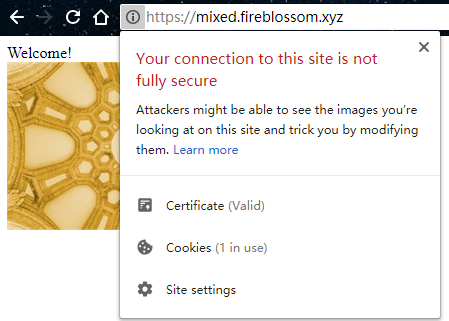
\includegraphics[height=3cm,width=7cm]{Figure/fig1.png}}%�ǵû���chrome�Ľ�ͼ
\caption{low-risk warning in chrome.}
\label{fig}
\end{figure}
this is probably because webmaster has configured his website correctly, including purchasing a valid certificate, but the website still contains images or scripts over plain HTTP. Although the browser was able to establish a valid HTTPS connection, there are still minor problems.

\subsubsection{Risk Level B: Medium-risk warnings that can be bypassed}
Bypassable HTTPS security warnings are the most common type of browser warning. Browsers use bypassable HTTPS security warning to treat the vast majority of HTTPS errors.
\begin{figure}[htbp]
\centerline{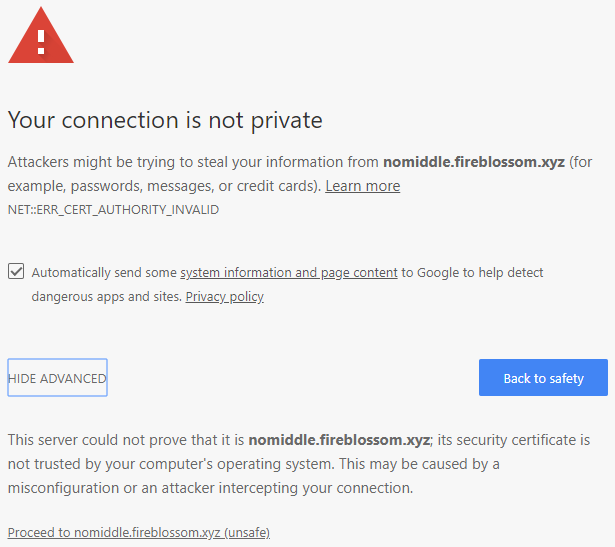
\includegraphics[height=3cm,width=7cm]{Figure/fig2.png}}
\caption{medium-risk warning in chrome.}
\label{fig}
\end{figure}
In this scenario, if there is an HTTPS error, the browser will stop the page load and display an HTTPS security warning. Typically, users are able to click through the warning by clicking on a button, but this may be disabled if the website servers the HTTP Strict Transport Security (HSTS) or HTTP Public Key Pinning (HPKP) header. Although the HTTP(s) traffic we captured through Fiddler[ https://www.telerik.com/fiddler] shows the web page is not transmitted in plain text, clicking through the warning may allow an actual man-in-the-middle attack to proceed.

\subsubsection{Risk Level C: High-risk warnings that cannot be bypassed}
As a worst case scenario, the browser will prevent uses from continuing to browse the website by showing a security warning that the users cannot bypass.
\begin{figure}[htbp]
\centerline{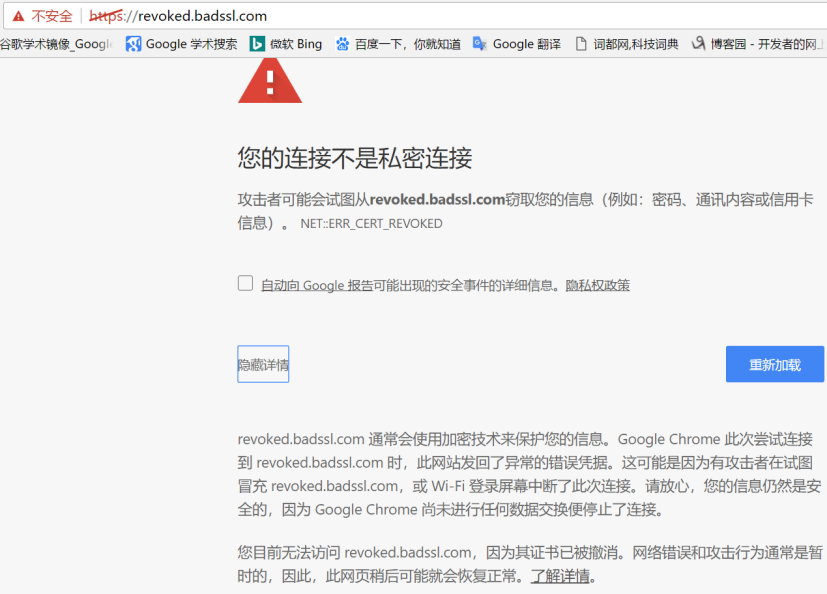
\includegraphics[height=3cm,width=7cm]{Figure/fig3.png}}%�ǵû����Լ�fireblossom.xyz��ַ�Ľ�ͼ
\caption{high-risk warning in chrome.}
\label{fig}
\end{figure}
this is probably because the website is supposed to establish a valid HTTPS connection, but the certificate chain fails to validate (e.g., a HTTPS certificate error occurs in a website that has deployed HSTS policy).

\subsubsection{Cannot establish HTTPS connection}
The browser may fail to establish a HTTPS connection to the server for unsupported TLS version, cipher mismatch, or other reasons. In this scenario, the browser cannot obtain certificates from the web server, let alone certificate validation, so the TLS handshake error is not discussed in this paper.
\begin{figure}[htbp]
\centerline{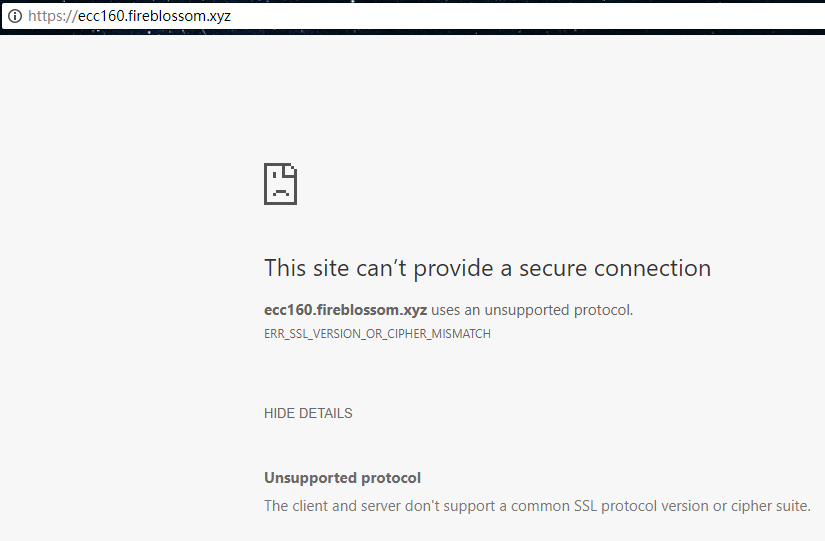
\includegraphics[height=3cm,width=7cm]{Figure/fig4.png}}%��ͼ��Ҫ�ٵ�����������
\caption{Cannot establish HTTPS connection in chrome.}
\label{fig}
\end{figure}

\subsection{HTTPS Errors}
%    In this subsection,
%    we focus on various types of errors that may trigger browser security warnings.
This section lists
the HTTPS errors of certificate verification of basic fields and extensions,
 name validation, and HTTPS security-enhancement.

\subsubsection{Basic Certificate Validation Error}
    Chain building Error occurs
    if the certificate chain presented by a web server
    cannot provide enough information for a browser to build a complete chain
    from the endpoint certificate to a trusted root certificate in the browser��s root store.

\textbf{Untrusted Root CA Certificate.}
    Untrusted root CA certificate means that 
        the root certificate of the certificate chain is not trusted by the browser.
%    This error occurs when the chain of intermediate CAs linking the server certificate to a root CA untrusted by browsers.
    
\textbf{Untrusted Self-signed Server Certificate.}
    Self-signed server certificate is a special case of root CA certificates. 
        %whose subject and issuer are the same.
    Similarly, self-signed certificate is not trusted by browsers and must be installed manually.
    
\textbf{Incomplete Certificate Chain.}
    Incomplete certificate chain means that 
    a complete certificate chain cannot be formed due to the lack of intermediate certificates.
    %In order to build a complete certificate chain,
    %browsers obtain the intermediate certificates in three ways.
    %First, the web server presents its server certificate accompany with all the necessary intermediate certificates that can leads to a trusted root certificate.
    %Second, browsers reuse the cached intermediate certificates.
    %Third, browsers actively fetch the missing intermediate certificates through an AIA field.
    %An incomplete chain error occurs, when all the attempts fail.

\textbf{Expired Certificate.}
    A certificate is only valid between its Not Before date and Not After date. An expired certificate error occurs if the Not After date is earlier than current time.

\textbf{Revoked Certificate.}
    For security reasons,
    CA can claim that a certificate is no longer valid before it expires by CRL, OCSP, and CRLset.
    A revoked certificate error occurs when the server uses a revoked certificate.

\textbf{Weak Signature Algorithm.}

    %The CA/Browser Forum allows RSA and ECC keys in certificates.
    %All RSA keys should be at least 2048 bits \cite{CAB2018BR},
    %and ECC keys should be at least 256 bits \cite{NIST2005ECC}.
    %A weak signature algorithm error occurs when the key length does not meet the requirements.

\textbf{Weak Digest Algorithm.}
    Weak Signature algorithm refers to the unsafe, collidable algorithm, such as SHA-1 \cite{Google2017sha1} and MD5 \cite{wang2004collisions}.
    %According to the CA/Browser Forum,
    %supported digest algorithms are SHA-256, SHA-384, and SHA-512. The SHA-1 and MD5 digest algorithm have been shown to be insecure, such as two different PDF files with the same SHA-1 hash \cite{Google2017sha1}.

\subsubsection{Certificate Extension Validation Error}
    In addition to the basic certificate validation, we also consider the certificate extension validation: Basic Constraints, Key Usage, and Extended Key Usage.

\textbf{Basic Constraints Extension.}
    The basic constraints extension consists of a "CA flag" and a PathLenConstraint.
    CA certificates must set the "CA flag" as true.
    PathLenConstraint is a non-negative integer, and it only works for CA certificates.
    The number of intermediate certificates between current CA and the server certificate cannot greater than PathLenConstraint.

\textbf{Key Usage Extension.}
    The key usage extension indicates the purpose of the public key contained in a certificate.
    According to RFC 5280 \cite{cooper2008rfc5280},
    all CA certificates must include "Certificate Signing" in their key usage extension, and
    all webhost certificates must include "Key Encipherment" in their key usage extension.

\textbf{Extended Key Usage Extension.}
    Extended key usage extension further refines key usage extension.
    If the extension is critical,
    all server certificates must include "serverAuth" in their extended key usage extension.


\subsubsection{Name Validation Error}
    Certificates are only valid for specific domain names.
    A name validation error occurs when domain names listed in a server certificate does not match the domain we visited.

\textbf{Domain Name Complete Mismatch.}
    Domain Name Complete Mismatch means that, there may be a complete mismatch between the domain name visited and the certificate received.
    For example, a user tries to visit www.baidu.com but gets a certificates for scholar.google.com.

\textbf{Common Name or Subject Alternative Name Mismatch.}
    Common Name (CN) and Subject Alternative Name (SAN) fields indicate the certificate subject identity information, and they are usually domain names.
    There are many kinds of errors with respect to CN and SAN, for example, CN does not match the domain name visited, SAN does not match the domain name visited, and the lack of CN/SAN.

\textbf{WWW Mismatch.}
    A www mismatch occurs when a user visiting www.example.com gets a certificates for example.com.

\textbf{Out-of-wildcard-scope Subdomain.}
    A out-of-wildcard-scope subdomain occurs when a user visiting a.b.example.com gets a certificates for *.example.com.


\subsubsection{HTTPS Security-Enhancement Error}
%\subsubsection{Certificate verification enhancement errors}
    In recent years, some security-enhancement policies have been added to HTTPS. We will focus on HSTS and HPKP errors.

\textbf{HPKP.}
%    HTTP Public Key Pinning (HPKP) \cite{Evans2015rfc7469} is used by web sites to instruct browsers to remember ("pin") the sites' public key over a period of time.
    A HPKP \cite{Evans2015rfc7469} error occurs when
    any public key of the certificate chain provided by the website
    does not match the pinned public keys.

\textbf{HSTS.}
    HTTP Strict Transport Security (HSTS) \cite{hodges2012rfc6797} directs browsers to interact with given sites only over HTTPS.
%    This policy is declared by web sites via the STS header field including three directives: max-age, includeSubDomains, and preload.
    An HSTS error occurs when a web site deploying HSTS has a certificate validation error.

\section{Browser Behaviors on HTTPS Errors}
%There are many community standards for certificate validation,
%    for example,
%    RFC 5246, RFC 6125, and RFC 5280.
%    The certificate validation in browser
%    is more than a  literal replication of Internet standards protocols.
%    It needs to balance security, standards, and user experiences.
\subsection{Goal and Methodology}
We attempt to analyze the browser security warnings
    on various HTTPS errors.
We register a domain name and
    establish the website for it by Nginx.
We induce different HTTPS errors
    by
    (\emph{a}) invalid or defective certificate chains in TLS negotiations,
    (\emph{b}) mismatched public keys after HPKP pins the public keys in browsers,
    and (\emph{c}) HTTP connections after the HSTS policy is activated.
Then, the evaluated browsers visit  the website one by one,
    and we record the browser behaviors.
We utilize OpenSSL to generate key pairs and some certificates,
    while some server certificates are applied from Let's Encrypt.
TLS 1.2 is adopted in the HTTPS connections.

%we register a domain name and resolve many subdomains to our web server, and
%    each subdomain has a certificate that violate one of the certificate constraints.
%    We use browsers to visit these domains and observe the browsers' behavior.
%All connections to the web server is encrypted and authenticated using TLS 1.2.


%�������̹������������Ѹ������������������������ҵķ�����IP������ʵ�鰲����������һ����ǩ���ĸ�CA����װ��CA��ϵͳ��������֣���ʹ�øø�CA��ÿһ��ʵ���֤�����ǩ��������ÿ��֤�飺1.����һ��˽Կ 2.����ʵ����������һ��OpenSSL�������ļ� 3.����֤������ 4.ʹ��OpenSSLǩ�� ��
%��½ʵ�����������װʹ��node.js�е�expressģ�齨��һ��web��������ָ���˿ڣ���װNginx��������ʵ���֤���ƶ������������༭Nginx�ķ�������Ϊÿ��֤������һ�������������������web�������˿ڣ�����Nginx����80��443�˿ڡ�
%�ֱ�ʹ��4�ֲ�ͬ�ں˵����������HTTPS�ķ�ʽ����ÿһ��ʵ���Ӧ������������������������ǰ���ͷ���������SNI��Ϣ���������˵�Nginx����������������SNI��Ϣ�ַ����Ӧ��������֤�飻������յ�֤�飬�ͷ�����������ɣ�����HTTPS���ӣ����������֤��Ͱ�ȫ���õIJ�ͬ������в�ͬ�ķ�Ӧ����ʵ�������м�¼��



%Our goal is to build a test harness that is able to determine whether a web browser reports HTTPS security warning for a variety of different kinds of HTTPS errors.

%we generate our own root certificate and install it so that the web browser trusts it.
%    This allows us to then generate and sign intermediate and leaf certificates as we wish.
%We implement out test as follows: for each test,
%    (1)generates a unique DNS name,
%    (2) uses OpenSSL to generate a test certificate that are syntactically well-formed but may violate one of the certificate constraints and internal dependencies that a valid certificate must satisfy.
%    (3)generate an Nginx server configuration for the test.
%Thus, each test has a dedicated DNS name and Nginx instance to serve the certificate chain.
%    We create a web page to present the browser certificate validation results.
 %   Thus, We can record whether the HTTPS security warning is triggered by such a combination of a test certificate and a HTTPS implementation.

The evaluated browsers are Chrome v67.0.3396.99,
 Firefox v62.0, Edge v42.17134.1.0, and IE v11.0.9600.17031 on Windows 10.
The results are summarized in Table I.
A, B, and C represent a warning of low-risk, medium-risk, high-risk, respectively.
D represent a fatal warning.
In order to find the browser behaviors on specified HTTPS errors,
   in each line of this table,
    we induce only one error in the certificate chains or HTTP headers,
    unless otherwise stated.
% A, B, C, and D represent low-risk, medium-risk, high-risk, and fatal warnings, respectively.

\begin{table*}[htbp]
\centering
\caption{Browser Behaviors on HTTPS Errors}
\begin{tabular}{p{2.55cm}|l|cccc}
\toprule
\multicolumn{2}{c|}{\multirow{2}{*}{HTTPS Errors}} & \multicolumn{4}{l}{Browser Security Warning} \\ \cline{3-6}
\multicolumn{2}{c|}{} & Chrome & Firefox & Edge & IE \\ \midrule[1pt]
\multirow{12}{*}{\begin{tabular}[c]{@{}c@{}}Certificate Verification\\of Basic Fields\end{tabular}}
 & Untrusted root CA certificate & B & B & B & B \\
% & Untrusted self-signed server certificate & B & \textcolor[rgb]{1.00,0.00,0.00}{B[xx]} & B & B \\     % ����Ӧ���е�ʲôר�ŵĽ���˵��
 & Incomplete certificate chain & B & B & B & B \\
 & Expired server certificate & B & B & B & B \\ \cline{2-6}
 & Revoked server certificate (via OCSP) & Secure & C & C & C \\
 & Revoked server certificate (via CRL) & Secure & Secure & C & C \\
 & Revoked server certificate (via CRLSet) & C & Secure & Secure & Secure \\ \cline{2-6}
 & Weak key (512-bit RSA key) & B & B & B & C \\
 & Weak key (1024-bit RSA key) & Secure & Secure & Secure & Secure \\
 & Weak key (160-bit ECC key) & D & D & D & D \\ \cline{2-6}
 & Weak hash algorithm (SHA-1) & B & B & Secure & Secure \\
 & Weak hash algorithm (MD5) & B & B & Secure & Secure \\ \midrule[1pt]
\multirow{17}{*}{\begin{tabular}[c]{@{}c@{}}Certificate Verification\\of Extensions\end{tabular}}
 & Server certificate &  &  &  &  \\
 & ~~incorrect cA flag (true), correct extensions of Key Usage and Extended Key Usage & Secure & B & Secure & Secure \\
 & ~~incorrect cA flag (true), incorrect extension of Key Usage (keyCertSign) & Secure & C & Secure & Secure \\
 & CA certificate &  &  &  &  \\
 & ~~incorrect cA flag (false) & C & B & C & C \\
 & ~~correct cA flag (true), incorrect PathLenConstraint & C & Secure & C & B \\ \cline{2-6}
 & server certificate &  &  &  &  \\
 & ~~no extended key usage, correct key usage & Secure & Secure & Secure & Secure \\
 & ~~no extended key usage, incorrect key usage & Secure & C & Secure & Secure \\
 & ~~no extended key usage, no key usage & Secure & Secure & Secure & Secure \\
 & ~~correct extended key usage, correct key usage & Secure & Secure & Secure & Secure \\
 & ~~correct extended key usage, incorrect key usage & Secure & Secure & Secure & Secure \\
 & ~~correct extended key usaget, no key usage & Secure & Secure & Secure & Secure \\
 & ~~incorrect extended key usage, correct key usage & C & C & C & C \\
 & ~~incorrect extendedKeyUsage, incorrect key usage & C & C & C & C \\
 & ~~incorrect extendedKeyUsage, no key usage & C & C & C & C \\
 & CA certificate &  &  &  &  \\
 & ~~incorrect key usage & C & C & C & C \\ \midrule[1pt]
\multirow{11}{*}{\begin{tabular}[c]{@{}c@{}}Name Validation\end{tabular}}
 & \textcolor[rgb]{1.00,0.00,0.00}{domain name complete mismatch} & B & B & B & B \\  % ���Ҳ��B����WWW mismatch��һ���������ʣ�Ӧ������
 & www mismatch & B & B & B & B \\
 & out-of-wildcard-scope subdomain error & B & B & B & B \\ \cline{2-6}
 & SAN and CN &  &  &  &  \\
 & ~~correct SAN, no CN & Secure & Secure & Secure & Secure \\
 & ~~correct SAN, \textcolor[rgb]{1.00,0.00,0.00}{incorrect CN} & Secure & Secure & Secure & Secure \\ % incorrect�ľ���������ʲô��
 & ~~incorrect SAN, no CN & B & B & B & B \\
 & ~~incorrect SAN, correct CN & B & B & B & B \\
 & ~~incorrect SAN, incorrect CN & B & B & B & B \\
 & ~~no SAN, incorrect CN & B & B & B & B \\
 & ~~no SAN, correct CN & B & Secure & Secure & Secure \\ \midrule[1pt]
\multirow{13}{*}{\begin{tabular}[c]{@{}c@{}}HTTPS Security\\Enhancement\end{tabular}}
 & HPKP: \textcolor[rgb]{1.00,0.00,0.00}{private store} &  &  &  &  \\      % ʲô��private/public store��Ҫ�к��ʵĽ��͡�
 & ~~first visit: incorrect HPKP header, second visit: correct/incorrect/no HPKP header & Secure & Secure & Secure & Secure \\
 & ~~first visit: correct HPKP header, second visit: incorrect/no HPKP header & Secure & Secure & Secure & Secure \\
 & HPKP: public store &  &  &  &  \\
 & ~~first visit: incorrect HPKP header, second visit: correct/incorrect/no HPKP header & Secure & Secure & Secure & Secure \\
 & ~~first visit: correct HPKP header correct, second visit: incorrect/no HPKP header & C & C & Secure & Secure \\ \cline{2-6}
 & HSTS: not preload list &  &  &  &  \\
 &~~some resouces over plain HTTP & A & A & A & A \\
 & ~~first visit: correct HSTS header, second visit: HTTPS error &C & C & C &C \\
 & HSTS: preload list &  &  &  &  \\
 & ~~some resouces over plain HTTP & A & A & A & A \\
 & ~~first visit: HTTPS errors & C &C & C & C \\ \bottomrule
\end{tabular}

  \label{tab:addlabel}%
  \vspace{6pt}

\leftline{``Secure" means that the browsers don't display any warnings.}
%\leftline{``B-\textgreater{}C" means that the policy will raise the original B-level warning to Level C.}

\end{table*}%




\subsection{Certificate Verification Errors of Basic Fields}
In these tests,
    the certificate extensions of Basic Constraints, Key Usage, Extended Key Usage and SAN,
        are correctly set.
The name in commonName also appears to be correct.

\textbf{Untrusted root CA certificate.}
We use OpenSSL to generate a certificate chain, %(whose cA flag is true, pathLenConstraint is null, key usage is keyCertSign),
 %   then use the root certificate to issue a valid server certificate (both CN and SAN of the server certificate contain the server's domain name, the key usage is keyEncipherment, extended key usage is serverAuth, and cA flag is false).
 and the root CA is not trusted by browsers.
%When visiting the website, We will receive the server certificate and a Level-B medium-risk warning with the error hint ``NET::ERR\_CERT\_AUTHORITY\_INVALID''.
All browsers show a Level-B warning on this error.
This warning is eliminated
 as we install the self-signed CA certificate in the root CA certificate store.
Chrome, Edge and IE rely on the Windows root CA certificate store,
     and Firefox uses its own NSS certificate store.



%%%%%%%%%%%%\textbf{Untrusted self-signed server certificate.}
%Basic Constraint = cA flag + pathLenConstraint
%%%%%%%We use OpenSSL to generate a self-signed server certificate
%%%%%%%    (who does not have Basic Constraint field, key usage is keyEncipherment and keyCertSign, extended key usage is serverAuth, and both CN and SAN of the self-signed server certificate contain the server's domain name).
%% Ӧ��˵��������root CA֮������֣�root CAҲ���Լ��İ�װ���̣�
%%%%%When we visit sites deploying self-signed server certificates, all four browsers display Level-B medium-risk warnings.
%%%%%After installing the self-signed certificates into the OS root store, Chrome, Edge, and IE consider it secure.
%%%%%%%%%The NSS root certificate store in Firefox does not accept self-signed server certificates, We need to avoid this warning by adding exception.

%chrome��ʾ�ľ�����NET::ERR_CERT_AUTHORITY_INVALID��Firefox��ʾ�ľ�����MOZILLA_PKIX_ERROR_SELF_SIGNED_CERT
%    After installing the self-signed certificates into the OS root store, Chrome, Edge, and IE consider it secure, but Firefox still displays a B-level (Medium-risk) warning.
%   Firefox has its own trust certificate store.
 %  First, click the ``Advanced" button on the warning page.
  % Second, click the ``Add Exception" button and confirm the domain name we added.
   %Third, click the ``Confirm Security Exception " button.
   %After all the steps have been completed, Firefox considers it secure.
%
%\textbf{Incomplete Certificate Chain.}
%\textbf{Expired Certificate.}

\textbf{Incomplete certificate chain, and expired server certificate.}
All browsers show Level-B warnings on an incomplete certificate chain, or expired server certificate.




\textbf{Revoked server certificate.}
In the certificate chain,
the server certificate is revoked and all CA certificates are not revoked.
(\emph{a}) OCSP. The server certificate is signed and revoked by Let's Encrypt.
    Let's Encrypt distributes the revocation status through OCSP.
Firefox, Edge, and IE show Level-C warnings,
    but Chrome considers it as secure.
(\emph{b}) CRL. When the server certificate is revoked through CRL,
 Chrome and Firefox consider it as secure, while Edge and IE show Level-C warnings \cite{liu2015end}.
(\emph{c}) CRLset. When the revoked server certificate is included in CRLset,
 Chrome shows a Level-C warning.

%\textcolor[rgb]{1.00,0.00,0.00}{    If a revoked certificate only contains available CRL field,
%        Chrome and Firefox consider it secure,
 %           but Edge and IE display C-level (High-risk) warnings.}
%%%%%%% û����ȷ˵������Dz����Ѿ��������ˣ������Լ�������OCSP��������CRLSet�У�����ô�����ģ�
%    If a revoked certificate only contains available OCSP field,
 %       Chrome considers it secure, but Firefox,
  %          Edge and IE display C-level (High-risk) warnings.
   % If a revoked certificate is only included in Chrome CRLset,
    %    Chrome displays a C-level (High-risk) warning,
     %       but Firefox, Edge and IE consider it secure.

%\textbf{Weak Signature Algorithm.}
\textbf{Weak key.}
%In this weak key paragraph, all server certificates are signed by SHA-256 with RSA Encryption.
 When receiving a server certificate binding a 512-bit RSA key pair,
    Chrome, Firefox, and Edge show Level-B warnings,
            while a C-level warning is shown in IE.
On a server certificate binding a 1024-bit RSA key pair,
    all browsers consider it as secure.
On a server certificate binding a 160-bit ECC key pair,
    all browsers show Level-D fatal warnings.

%\textbf{Weak Digest Algorithm.}
\textbf{Weak hash algorithm.}
%In this weak hash algorithm paragraph, all server certificates are signed by RSA and the public key of server certificates are 1024-bit RSA key.
    When receiving a server certificate signed by SHA-1 or MD5,
        Chrome and Firefox display Level-B warnings,
            but Edge and IE consider it as secure.
\subsection{Certificate Verification Errors of Extensions}
In these tests of certificate extensions,
    the certificate chain consist of one self-signed root CA certificate, an intermediate certificate, and the server certificate.
The root CA certificate is installed in the browsers' certificate store.

\textbf{Basic Constraints extension.}
If the cA flag of the Basic Constraints extension is true in the server certificate
    while the key usage is set as a common TLS server certificate (i.e.,
    the Key Usage extension is keyEncipherment, and the Extended Key Usage extension is serverAuth),
% whose cA flag is incorrect (cA flag is true), but other fields is correct (key usage is key Enpherment, extended key usage is serverAuth),
    Chrome, Edge, and IE consider this certificate chain as secure,
    but Firefox shows a Level-B warning.
%
If the cA flag is true in the server certificate
    while the key usage is set as a common CA certificate (i.e.,
        the Key Usage extension is keyCertSign, and no Extended Key Usage extension),
    Chrome, Edge, and IE consider it as secure,
    but Firefox shows a Level-C warning.

As long as the cA flag is false in the intermediate CA certificate,
    whether the key usage is set as a CA certificate or a TLS server certificate,
Chrome, Edge, and IE show Level-C warnings,
     and Firefox shows a Level-B warning.
     %\textcolor[rgb]{1.00,0.00,0.00}{Firefox's NSS root store does not accept a certificate whose CA flag is false, so we does test the Firefox for this HTTPS error.}  % Ӧ��ʹ�ö༶֤�飻root CA��flag��ȷ���м�CA��flag���󣬵�����֤�飡
%If the cA flag is false in the intermediate CA certificate
%    while the key usage is set as a common TLS server certificate,
%    the results are the same.
That is, if a TLS server holds a certificate where the cA flag is false,
 it can issue certificates for any domain names to launch MitM attacks,
 because Firefox only shows bypassable Level-B medium-risk warnings.

If the server certificate is signed by a CA certificate that has a correct cA flag (cA flag is true)
    but does not conform to PathLenConstraint (the PathLenConstraint of self-signed root CA certificate is 0),
    Chrome and Edge display Level-C high-risk warnings,
    Firefox consider it secure, and IE displays a Level-B medium-risk warning.


\textbf{Key Usage and Extended Key Usage.}
    We didn't designate key usage and the extend key usage as critical or non-critical.
    If a server certificate has extended key usage field including serverAuth, no matter what the key usage is,
        all the four browsers consider it secure.
    If a server certificates has extended key usage field not including serverAuth, no matter what the key usage is,
        all the four browsers display Level-C high-risk warnings.
    If a server certificates does not have extended key usage field, and its key usage field is correct or does not have key usage field,
        all the four browsers consider it secure.
    If a CA certificate has incorrect key usage field,
        all the four browsers display Level-C high-risk warnings.

\subsection{Name Validation Errors}
    For domain name complete mismatch, www mismatch, and out-of-wildcard scope subdomain error,
    all four browsers display Level-B medium-risk warnings.

Next, SAN or CN incorrect means domain name complete mismatch.
    For correct SAN, no matter what the CN is, all the four browsers consider it secure.
    For incorrect SAN, no matter what the CN is, all the four browsers display Level-B medium-risk warnings.
    If the server certificate does not have SAN field, and the CN field is incorrect, all the four browsers display Level-B medium-risk warnings.
    If the server certificate does not have SAN field, and the CN field is incorrect,
    Chrome displays a Level-B medium-risk warning,
            but Firefox, Edge, and IE consider it secure.

\subsection{HTTPS Security-Enhancement Errors}
\textbf{HPKP.}
``private store" means that the root certificate of the certificate chain is installed  manually by the user to the browsers' trust root store.
    In this paragraph, the root certificate is generated by OpenSSL.
``public store" means that root certificate of the certificate chain is trusted by browsers.
    In this paragraph, the root certificate is from Let's Encrypt.

Edge and IE don't support HPKP, so they don't display any warnings on HPKP errors.
    Chrome and Firefox have the same behaviors on HPKP validation.

%    Next, let's look at the warning behaviors of Chrome and Firefox.
%If the root certificate of the certificate chain is installed manually by the user, no HPKP errors will be warned.
If the root certificate is from private store, no HPKP errors will be warned.
    If the root certificate of the certificate chain is from public store, there are two scenarios.
        (1)We received an incorrect HPKP header when we visit the website for the first time, such as nonnumeric max-age, pin-sha256 mismatch,
        then when we visit the website for the second time, no HPKP errors will be warned.
        (2)We received a correct HPKP header when we visit the website for the first time,
        then when we visit the website for the second time,
            if no certificate in the certificate chain matches the first time pinned certificates,
        a HPKP error will be warned, Chrome and Firefox will display Level-C high-risk warnings.


%correct HPKP header����˼��˵, HPKP header��ѭRFC7469�Ĺ涨��HPKP header������������pin-sha256��һ����֤�����ϣ�һ������֤������,max-age��ֵ��һ������


%HPKP�﷨Public-Key-Pins: pin-sha256="base64=="; max-age=expireTime [; includeSubDomains][; report-uri="reportURI"]
%Chrome���public store�е�֤�����HPKP ���
%��Pin header = 1��֤�����е�֤��
%������
%��Pin header = 1������֤�����е�֤��
%������
%��Pin header = 2������֤�����е�֤��
%������
%�ܵ�һ�η���ʱpin header = ֤�����е�Cert A &��֤�����е� backup cert��
%��֤��A���͸����������A�������м�CA��������ĩ��֤�飩
%�ڶ��η���ʱpin header = ֤�����е�Cert A &��֤�����е� backup cert��
%��backup certificate���͸������
%�Ỻ�棬������
%��Max-age����Ϊ0������������ֵ
%������
%�޵�һ�η���ʱpin header = ֤�����е�Cert A &��֤�����е� backup cert��
%��֤��A���͸����������A�������м�CA��������ĩ��֤�飩��
%�ڶ��η���ʱpin header = backup cert & ��֤�����е�C��
%��backup certificate���͸��������
%�����η���ʱ��������pin header����Cert A���͸�browser
%�����η���ʱ��������������backup & C
%�ߵ�һ��Pin header = A & B������A�������
%�ڶ��β�����pin header������A�������
%�����������滹��
%���һ��pin header = ֤�����е�Cert A &��֤�����е� backup cert
%����A���������
%�ڶ���pin header = Cert A & C������C�������
%�ᱨ�����������ǵ�һ�ε�pinֵ
%�ܽ᣺ֻ�е�һ��pin�ԣ��ڶ���pin����ʱ��Żᱨ��������ʱ�򶼲�����



 \textbf{HSTS.}
 HSTS is a trust-on-first-use policy, but HSTS has a preload list in the browsers.
 Whenever visiting the domain name in the preload list,
    the browser will only use HTTPS to initiate the connection.
 This list is maintained by Google Chromium and is used by mainstream browsers like FireFox, Edge and IE.


    Whenever you visit a website in the HSTS preload list, % ʲô��preload list��Ӧ���н��͡����ڵĽ������������Ī�����
    if the website has HTTPS error including incomplete certificate chain, expired certificates, or any other Level-B medium-risk HTTPS errors mentioned in this paper,
    all the four browsers will display Level-C high-risk warnings.
        %all the four browsers display C-level (High-Risk) warnings on B-level (Medium-Risk) HTTPS errors,
    All the four browsers display Level-A low-risk warnings on websites that transmit some resources over plain HTTP.

    When we visit a website not in the HSTS preload list,
        if we received an correct HSTS header when we visit the website for the first time,
        then when we visit the website for the second time encountering Level-B medium-risk HTTPS errors mentioned in this paper,
        all the four browsers display Level-C high-risk warnings.
        All the four browsers display Level-A low-risk warnings on websites that transmit some resources over plain HTTP.

%The site's certificate must first be trusted by the browser, including server authentication and certificate/certificate chain verification. We first pin the sha256 value of the intermediate CA and any other sha256 value into the header, and the browser will cache the two sha256 values ??and verify them in the next access within the cache effective time. If the two sha256 values ??of the pin are in the same certificate chain, they will not be cached and will not prompt any errors.

%If the next time the certificate issued by the site is valid and the certificate is in the pin list, the HPKP cache will be refreshed, including the SHA-256 value of the pin and the cache validity period, whichever comes first. If the intermediate CA of a certificate chain that a webmaster plans to replace is not in the current pin, you should keep using the original certificate or the alternate certificate and change the value of the other pin until the longest cache time, you can safely delete the old certificate's Pin.

%In a site with HPKP cache and in effect, if the certificate received when accessing the site is a certificate in the public certificate store, and the certificate chain is not in the pin, it will be reported by the browser, but can be ignored. If the visited site is in a private certificate store, ie a self-signed certificate chain, no errors will be reported even if the certificate does not comply with the HPKP policy, and the HPKP settings cache will not be updated.

%The cache of the HPKP policy has no relationship with the storage area where the certificate is located. If the certificate is legal in the browser and does not conflict with the pin in the cache, the sha256 value of the self-signed certificate chain is also stored in the pin of the HPKP policy.

%When the site has the HSTS header set and is not in the preloaded list, the first visit to the site does not force https access. When the local browser has the HSTS setting cache, the browser will make a jump inside the browser when accessing the http site without initiating an HTTP network request.

%\begin{figure}[htbp]
%\centerline{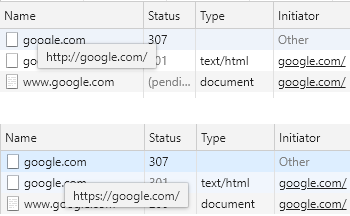
\includegraphics{Figure/fig5.png}}
%\caption{Network requests to access a site with HSTS.}
%\label{fig}
%\end{figure}

%The cache obtained by the browser through the HSTS response header is stored in the dynamic HSTS, and the site in the preloaded list is in the static storage area, which cannot be modified after the browser is compiled. However, the HSTS policy is stored in two areas and has no effect on the validity of the settings.

%The HSTS policy only takes effect in the risk alert that the browser can skip. It will block the option to ignore the error, and the browser will also prompt "Cannot continue browsing due to the HSTS policy." For low-risk prompts (Level A), the browser can still access the site normally, and there will be an exclamation point prompt, which is no different from the prompt without the HSTS policy. Naturally, there is no change to the risk alert (Level C) that could not be skipped.


\section{Discussion and Suggestion}
%In the experiment, we found that different browsers have different processing methods for some unsafe scenarios.
%Through comparison between them, we have summarized the existing risks of several browsers.

In this section,
    we discuss the browser defects on handling HTTPS errors,
    and present some suggestions.

\subsection{Weak Cryptographic Algorithm}
The following cryptographic algorithms are publicly prohibited or unrecommended \cite{CAB2018BR, NIST2005ECC},
but the processes of browsers can lead to (\emph{a}) forged certificates to be accepted
  or (\emph{b}) broken key pairs to be used in TLS negotiations.

The collisions of MD5 and SHA-1 have been found \cite{wang2004collisions, sha1-collision},
    and the weakness of MD5 was exploited to successfully forge certificates \cite{md5-forged-cert1, md5-forged-cert2}.
%Several security incidents have shown that,
%        attackers can use SHA-1 and MD5 to colliding fraudulent certificates,
However, Edge and IE do not show any warnings on certificates signed by MD5 or SHA-1.

The first factorization of 512-bit RSA was finished in 1999 \cite{cavallar2000factorization},
    and an 512-bit RSA key pair is broken in four hours using the Amazon EC2 platform in 2016 \cite{DBLP:conf/fc/ValentaCLFBH16}.
However, Chrome, Edge, and IE show only \emph{bypassable} Level-B warnings on 512-bit RSA.
%On the contrary,
 %   these browsers show Level-D fatal warnings on a server certificate with 160-bit ECC key pair,
  %   which is stronger than 512-bit RSA \cite{ecc-vs-rsa}.
%1024-bit RSA is expected to be broken within 2015 to 2020 \cite{Berlin2017An},
%1024-bit RSA is expected to be phased out.
%1024-bit RSA can be broken now at a cost ranging from tens of thousands to hundreds of millions of dollars,
%1024-bit RSA is at the greatest risk,
1024-bit RSA is now expected to be broken at a cost ranging from tens of thousands to hundreds of millions of dollars  \cite{NIST2016Post-Quantum},
    but none of the evaluated browsers show any warnings on certificates with 1024-bit RSA.

\subsection{Certificate Revocation}
Most certificates in the Internet are revoked through CRL and/or OCSP,
    but CRL and OCSP are not supported by Chrome while Firefox does not support CRL.
The statistics in 2015  \cite{liu2015end} show that,
    99.9\% of server certificates contains a CRL distribution point, and
%        however, Chrome and Firefox don't display any warnings on revoked server certificates through CRL.
%        we think Chrome and Firefox need to be improved on this.
%
    95\% contains an OCSP responder.
%        however, Chrome does not display any warnings on revoked server certificates through OCSP.
%        we think Chrome need to be improved on this.

Chrome checks the revocation status
    only through CRLSet \cite{CRLSet}.
%        and Chrome only displays warnings on revoked certificates through CRLSet.
%Although CRLset is constantly updated,   in our tests,
%     Chrome still consider the HTTPS visits as secure \textcolor[rgb]{1.00,0.00,0.00}{within a month} after the server certificate was revoked. %% ��û�и���׼ȷ��ʱ�䣿
%This certificate is issued by Let's Encrypt and the serial number is 03e37c58091fb4056aa84130a1e54f8b58fd.
%        we think Chrome need to be improved on this.
So a compromised key pair can still be exploited to launch MitM or impersonation attacks after the certificate is revoked through CRL and OCSP,
        and the attacks will probably succeed in Chrome for CRLSet covers only 0.35\% of all revocations in the Internet \cite{liu2015end}.

\subsection{Certificate Extension}
%\textbf{Basic Constraints.}
The Basic Constraints extension is defined to distinguish CA certificates and non-CA ones \cite{cooper2008rfc5280}.
However,
    when the server certificate is verified by a certificate in which the cA flag is false,
    i.e., a non-CA entity acts as CAs to sign server certificates
        for any domain names to launch attacks,
            Firefox shows only bypassable Level-B warnings.
Moreover, Firefox does not process the pathLenConstraint field correctly,
    and the violated pathLenConstraint does not trigger warnings in Firefox.
These defects can be exploited to launch successful MitM and impersonation attacks.

If a CA acts as the TLS server in HTTPS,
    i.e., the cA flag in the ``server'' certificate is true,
Chrome, Edge and IE consider it as secure and show no warning.
However, %in our opinion,
    such configurations are rather uncommon,
    and Level-A warnings shall be suitable.

%\textbf{Extended Key Usage and Key Usage.}
If a certificate contains the extensions of Key Usage and Extended Key Usage,
    two extensions must be processed independently,
    and the certificate is only used for the purpose(s) consistent with both extensions  \cite{cooper2008rfc5280}.
%If there is no purpose consistent with both extensions, then the certificate MUST NOT be used for any purpose \cite{cooper2008rfc5280}.
This rule is not complied with in Chrome, Edge and IE:
    when the server certificate includes only the keyCertSign usage and the serverAuth extended usage,
     no warning is shown.
%
Chrome, Edge, and IE do not process the Key Usage extension correctly,
    even if it is marked as critical:
no warning is shown when the TLS server certificate does not include the keyEncipherment usage.
%However,
%    these browsers process the \emph{non-critical} Extended Key Usage extension correctly:
%    when the server certificate does not include the serverAuth extended usage,
%    Level-C warnings are shown.
So a certificate for other purposes may be maliciously used in HTTPS, and accepted by these browsers.

% If a certificate contains both a key usage extension and an extended
%   key usage extension, then both extensions MUST be processed
 %  independently and the certificate MUST only be used for a purpose
  % consistent with both extensions.  If there is no purpose consistent
   %with both extensions, then the certificate MUST NOT be used for any
   %purpose.(RFC 5280)
\subsection{Name Validation}

All browsers show bypassable Level-B warnings on different name validation errors:
complete mismatch,
WWW mismatch and out-of-wildcard-scope subdomain.
However,
%    in our opinion,
    these errors bring very different levels of risk,
    and it is practicable to show a higher-level warning on complete mismatch
     because low-cost TLS server certificates are available.


%The CA/Browser Forum suggests that
%    deprecates the CN field and lists applicable names in SAN field.
The browsers behave inconsistently in name validation.
Chrome checks the domain name \emph{only} in the SAN extension.
Firefox, Edge, and IE consider a server certificate as secure,
    if it contains correct CN but no SAN;
    on the contrary, it triggers Level-B warnings in Chrome.
This may lead to a problem of usability:
    a legitimate certificate considered as secure by other browsers,
    may trigger a warning in Chrome.



\subsection{HSTS}
%HSTS is supported by all evaluated browsers.
The visits over plain HTTP that definitely violates the HSTS policy,
 trigger only Level-A warnings, not interrupting the user's browsing.
If the HSTS policy is enforced by the pre-loaded list, which is manually configured by the user,
    the user shall be explicitly notified on such visits over HTTP.
If HSTS is enforced  by the HSTS header, which is sent by the website,
    such visits over plain HTTP are probably initiated by attackers because the website itself does not allow HTTP visits.

\subsection{HPKP}
HPKP is supported only in Chrome and Firefox.
        Chrome and Firefox do not conduct HPKP validation
            when the certificate chain is verified by a user-installed root CA certificate.
So a website cannot enhance its HTTPS security by HPKP,
    unless it applies for a certificate from the publicly-trusted CAs.
 %   Thus, If a malware installs its root certificate on the user's computer,
 %       it may defeat the protections of HPKP and successfully launch the man-in-the-middle attack.

%To enable certificate chain validation, Chrome has access to two stores of trust anchors: certificates that are empowered as issuers. One trust anchor store is the system or public trust anchor store, and the other other is the local or private trust anchor store. The public store is provided as part of the operating system, and intended to authenticate public internet servers. The private store contains certificates installed by the user or the administrator of the client machine. Private intranet servers should authenticate themselves with certificates issued by a private trust anchor.

%Chrome does not perform pin validation when the certificate chain chains up to a private trust anchor. A key result of this policy is that private trust anchors can be used to proxy (or MITM) connections, even to pinned sites. ��Data loss prevention�� appliances, firewalls, content filters, and malware can use this feature to defeat the protections of key pinning.
% We deem this acceptable because the proxy or MITM can only be effective if the client machine has already been configured to trust the proxy��s issuing certificate �� that is, the client is already under the control of the person who controls the proxy (e.g. the enterprise��s IT administrator). If the client does not trust the private trust anchor, the proxy��s attempt to mediate the connection will fail as it should.

%In order to control the browsing behavior of the internal network, some companies often pre-set the self-signed certificate in the computer in the office area, and replace the HTTPS connection certificate in the gateway to obtain the information contained in the HTTPS traffic, detect and prevent the information leakage inside the company, which is a typical MITM attack. Some malware may also use the same way to attack a personal computer. Many computer applications will trigger the UAC of the Windows system during installation. After clicking and agreeing, the computer settings can be modified. After the malware spoofs the user's consent, you can modify the computer settings, such as burying your own root certificate. Eavesdrop on all traffic through a self-signed certificate and send sensitive information to the attacker.




%\section{Suggestions}
%
%\subsection{Do not use a self-signed CA certificate}
%
%Trusted root certificates on the Internet have very strict protection measures, such as offline protection.But users may store the seif-signed CA's private key on the local computer, and may even be exposed on the Internet, such as send by email. This will greatly Increase the risk of CA private key disclosure. The attacker can obtain a fake certificate that is completely legal and extremely difficult to distinguish for the user. The only difference between the attacker and the real certificate may be that the public key, the serial number and the signature value are different and difficult to be discovered. In this case, the possibility of being attacked is very high. We recommend not issuing a CA certificate when using a self-signed certificate.
%
%We did not find a way to directly add a endpoint certificate to Firefox's certificate store(Section 5.2). So try to avoid using self-signed certificates in Firefox browser.
%
%\subsection{Minimize the validity period of the certificate}
%For personal websites, the revoked certificate is not detected by Chrome(section 5.3), and Chrome is one of the most popular browsers. A workable approach is to minimize the validity of the certificate and update the certificate regularly.




%HTTPS errors�½ڶ��Dzο��������������ϣ�����������


{\footnotesize \bibliographystyle{IEEEtran}
\bibliography{vSSL}
}





\end{document}
